\documentclass[12pt, a4paper]{article}
\usepackage{titlesec}
\usepackage{graphicx}
\usepackage{amsmath}
\renewcommand{\figurename}{Att.}
\titlelabel{\thetitle.\quad}
\author{Pēteris Račinskis pr20015}
\begin{document}
\title{4. mājas darbs}

\maketitle

\section{Uzdevums}

Dots koka $G$ Prūfera kods $P=(1,1,3,3,1,1,8,5,7)$. Atjaunoto koku $G' = (V',E')$ iegūst, sākot no koda beigām  ar 
\begin{equation}
    V'_0 = \max(V[G])
    \end{equation}
    \begin{equation}
    E'_0 = \lbrace \lbrace \max(V[G] \setminus V'_0), P_{n-2} \rbrace \rbrace
    \end{equation}
un katram elementam izpildot soļus
\begin{equation}
    v_i = 
\begin{cases}
    P_{n-i-1}, \text{ ja } P_{n-i-1} \notin V'_{i-1} \\
    \max(V[G] \setminus V_{i-1})
\end{cases}
\end{equation}
\begin{equation}
    V'_i = V'_{i-1} \cup v_i
\end{equation}
\begin{equation}
    E'_i = E'_{i-1} \cup \lbrace v_i, P_{n-i} \rbrace
\end{equation}
Process attēlots grafiski:

\begin{figure}[h!]
    \centering
    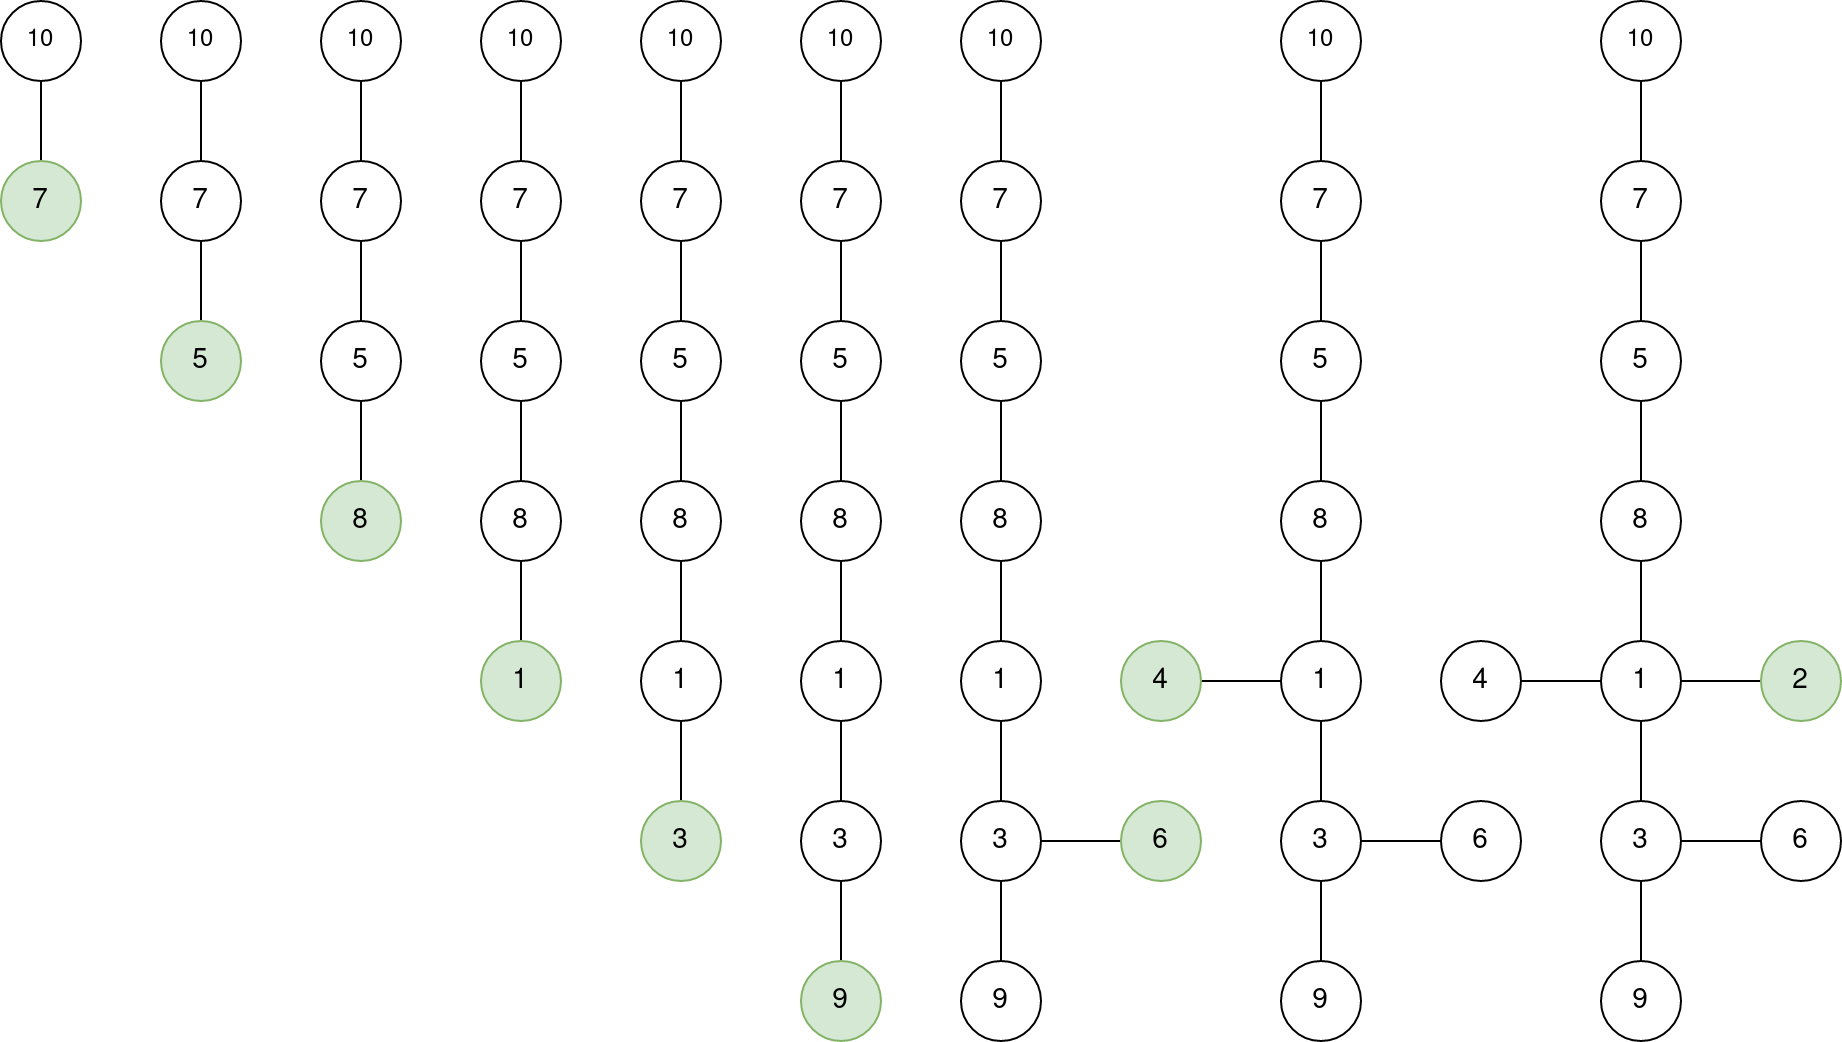
\includegraphics[height=4.8cm,page=1]{pruefer.png}
    \caption{Koka atjaunošana pēc Prūfera koda}
    \label{fig:att}
\end{figure}

\newpage
\section{Uzdevums}

asfasf

\section{Uzdevums}

asfaf

\end{document}